\begin{figure}
  \centering
  % 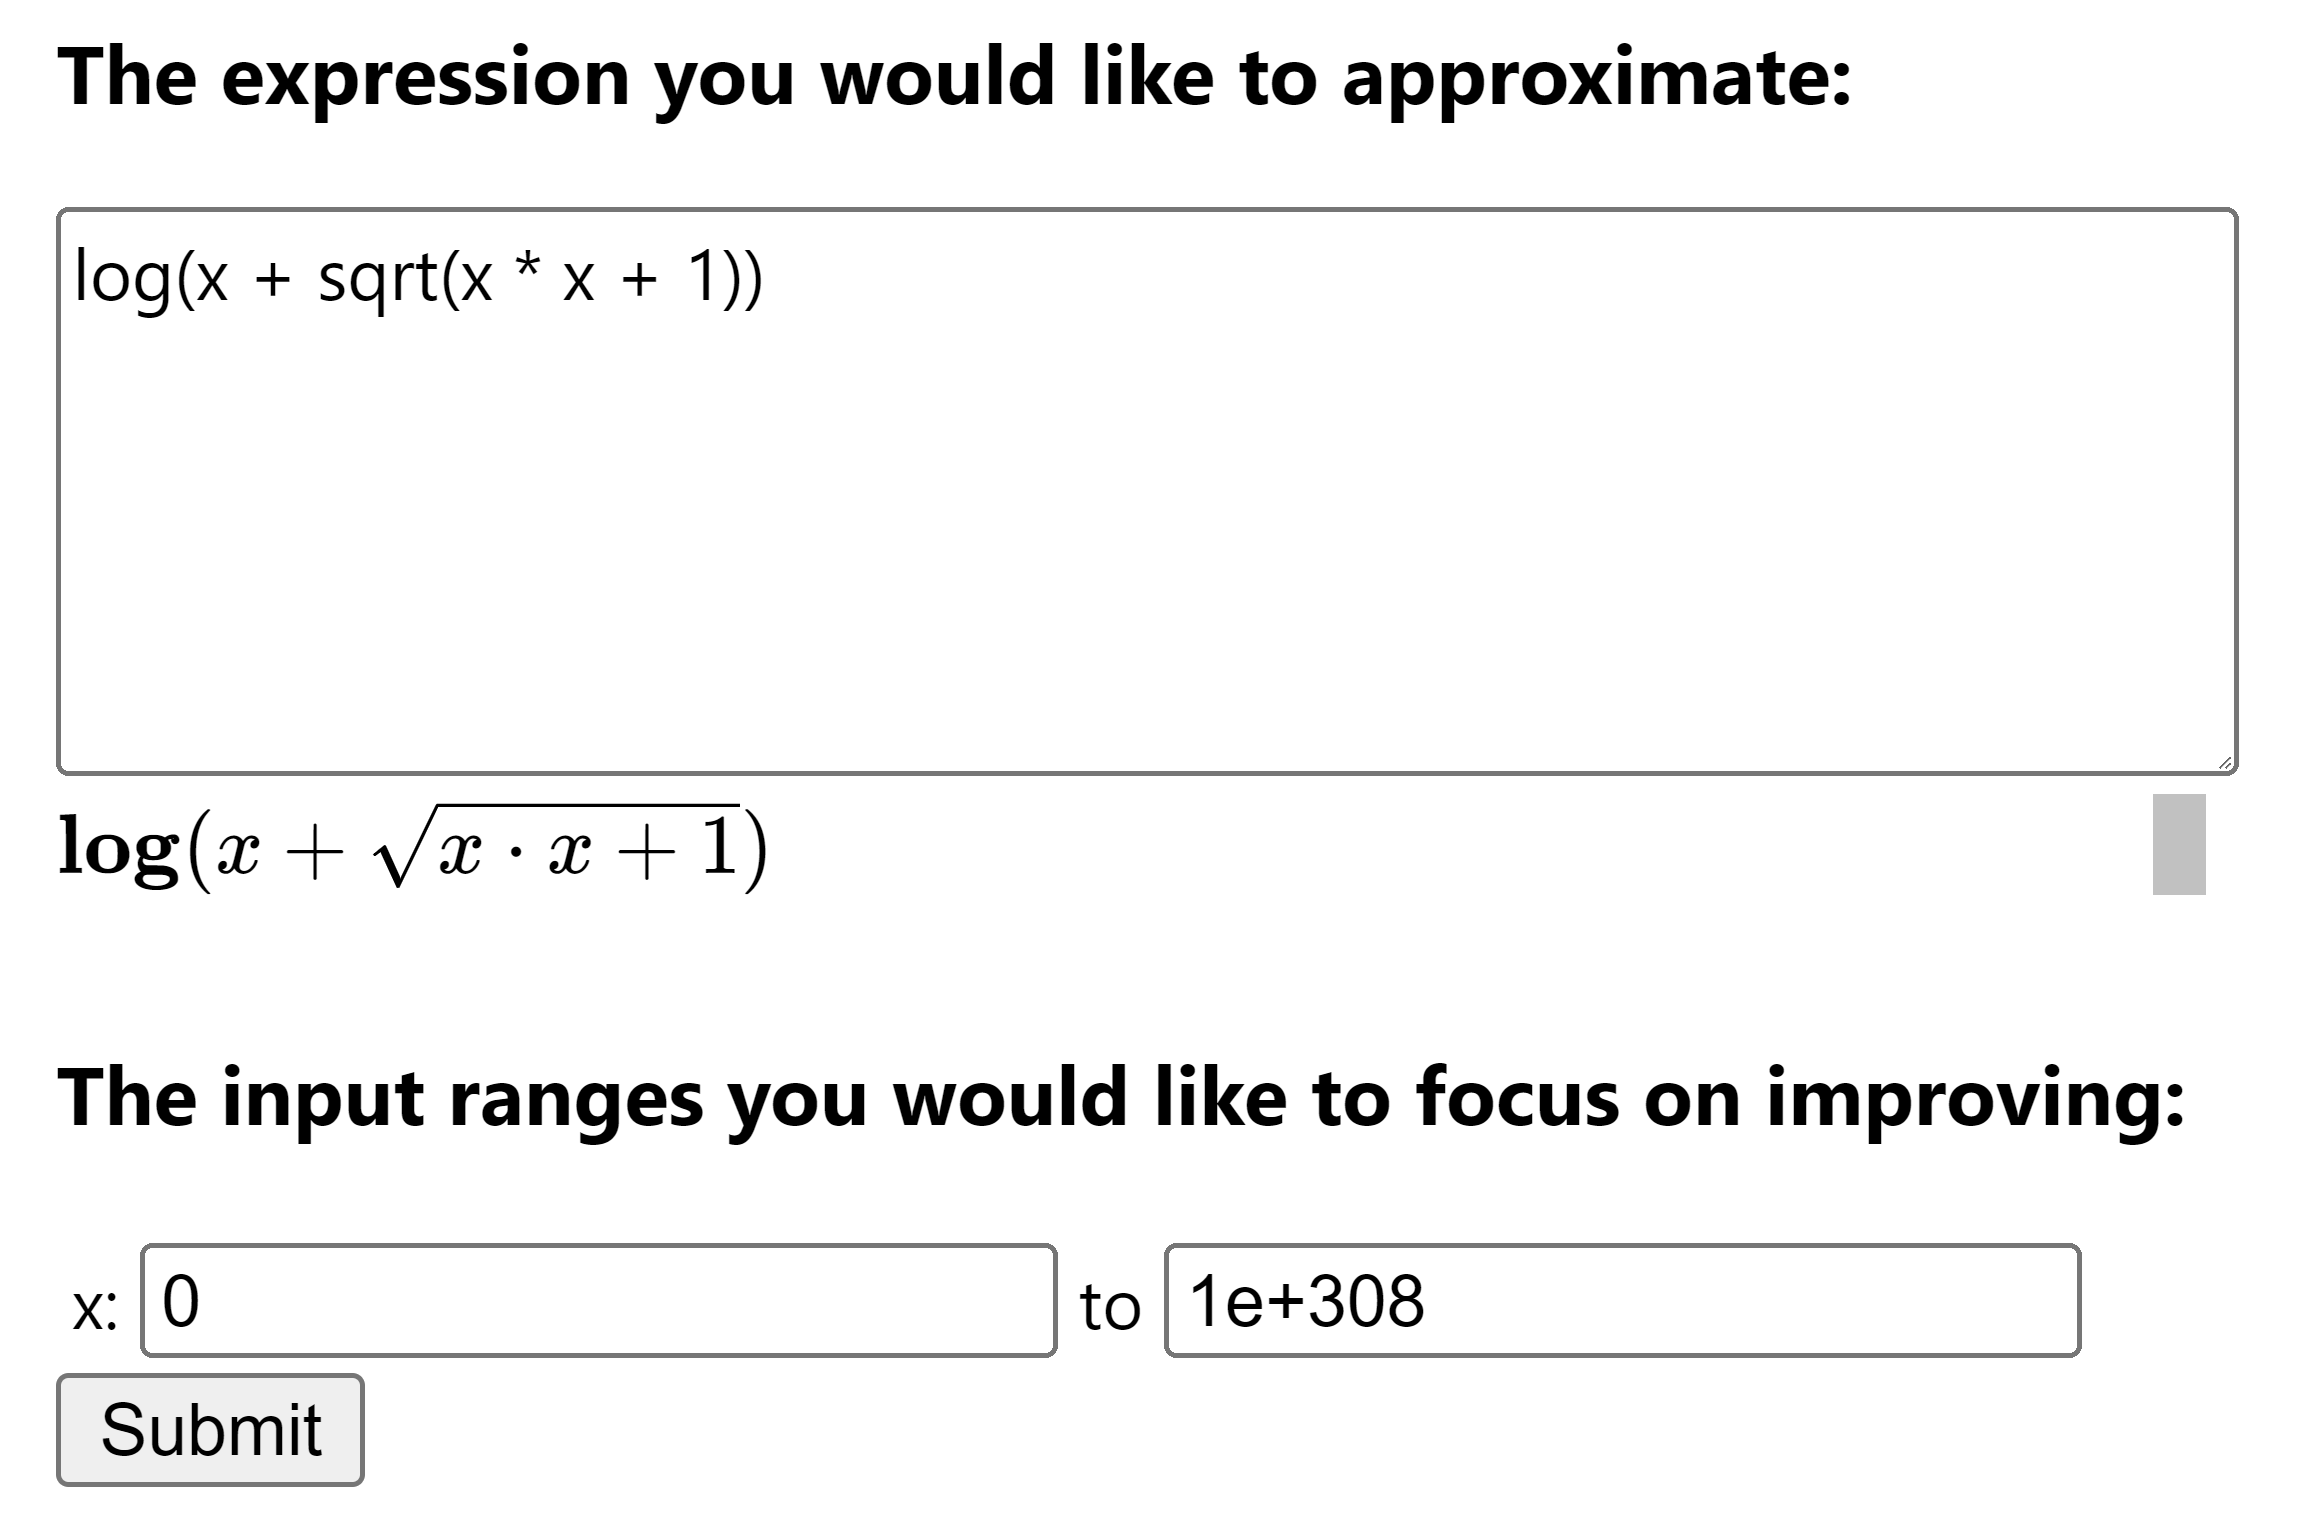
\includegraphics[width=\linewidth]{figures/new-tab.png}
  \shadowimage[width=\linewidth]{figures/new-tab.png}
  \caption{Users enter a new expression.}
  \label{fig:new-tab}
\end{figure}

\begin{figure*}
  \centering
  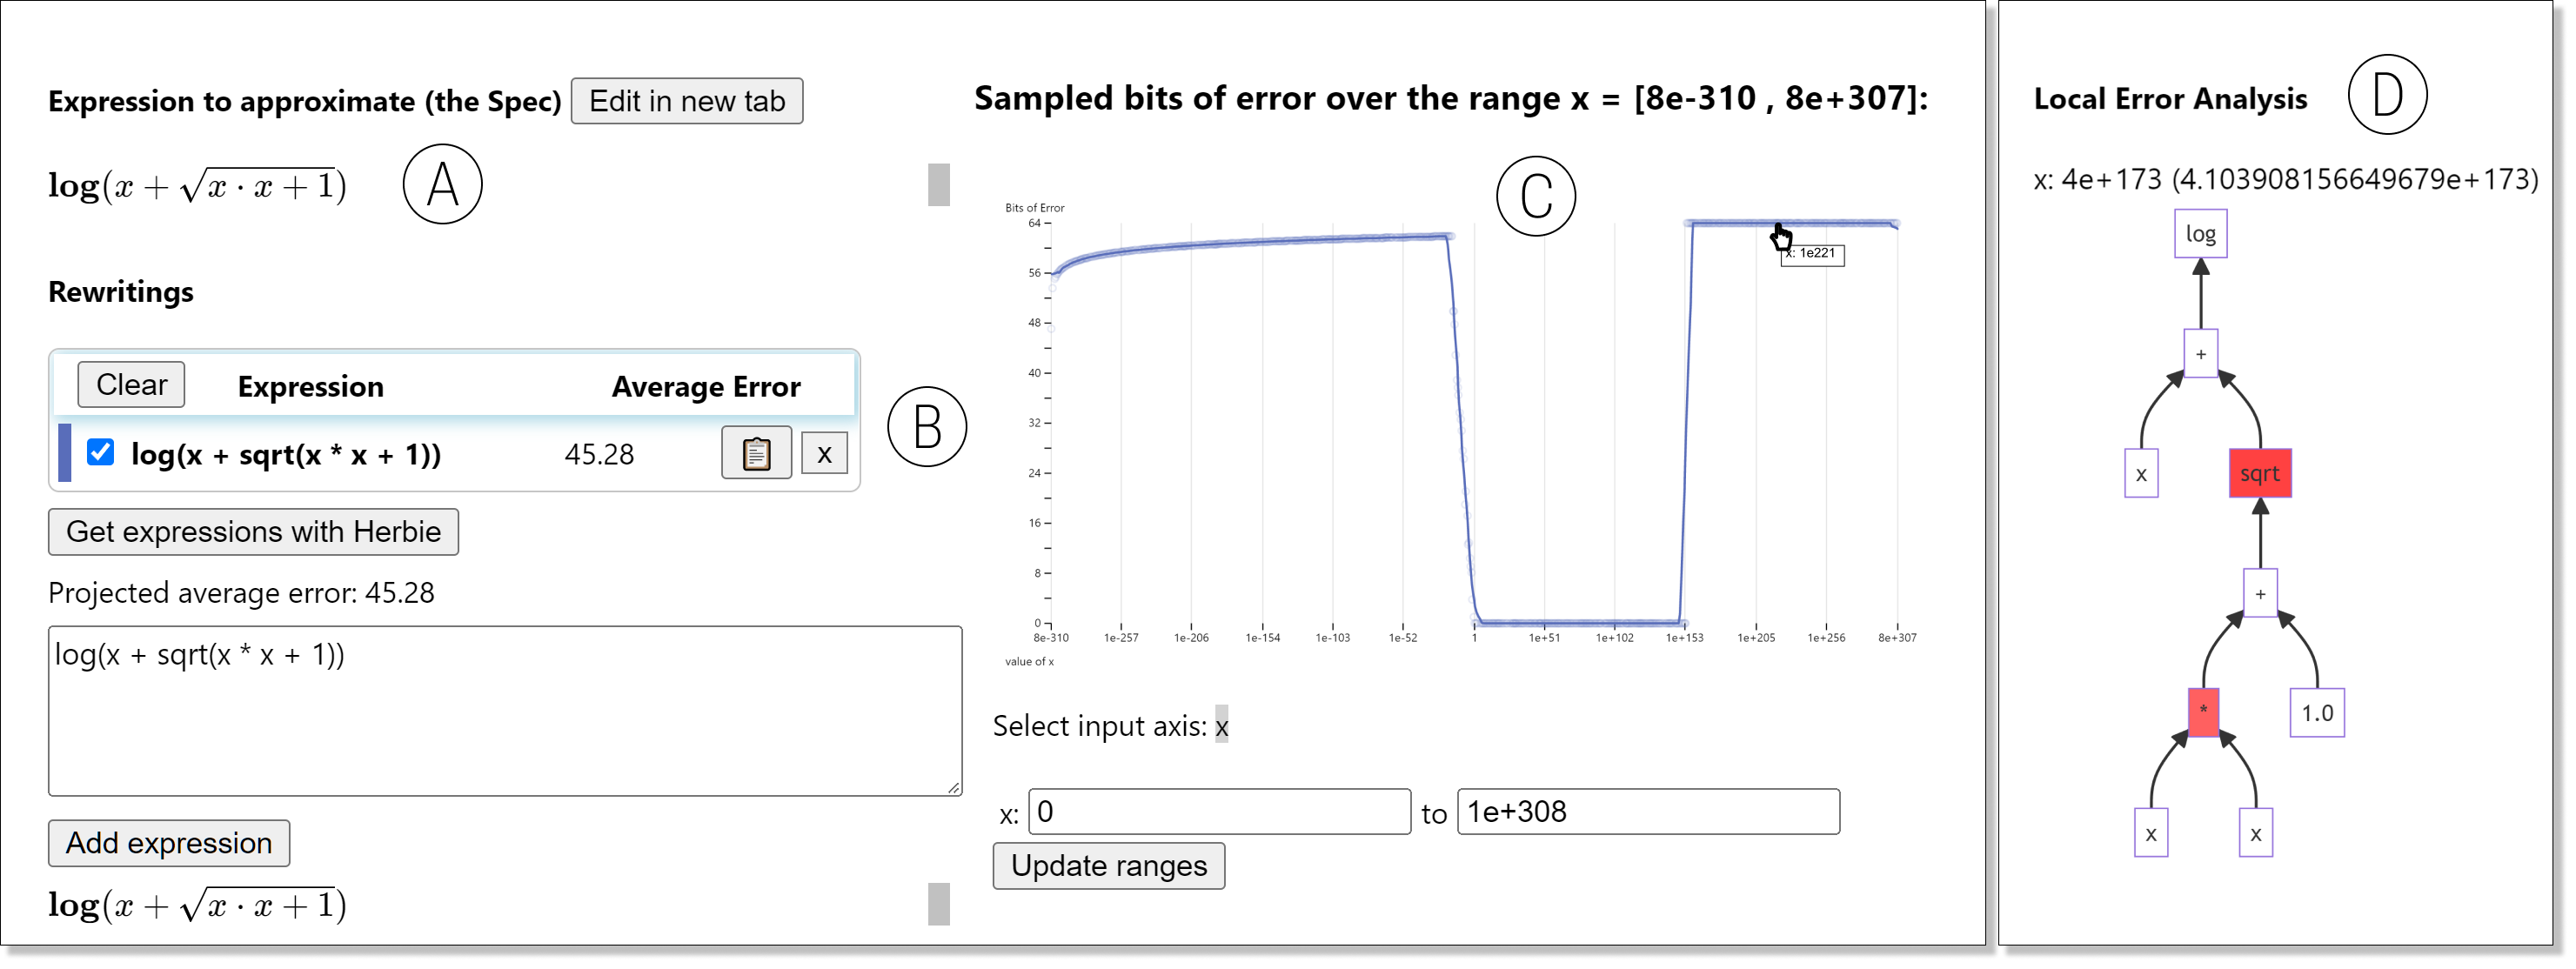
\includegraphics[width=\linewidth]{figures/diagnosis.png}
  \caption{Diagnosis.
  The specification (A) shows the expression the user is trying to implement.
  The rewritings table (B) shows the expressions the user has tried.
  The error plot (C) shows the error of the current expression.
  The local error heatmap graph (D)
    shows the error breakdown of the currently selected point.
  }
  \label{fig:diagnosis}
\end{figure*}

\begin{figure}%
  \centering
  \shadowimage[width=.8\linewidth]{figures/expression-details.png}
  \caption{The Expression Details view shows 
  a LaTeX rendering and plain text to help users 
  understand and work with the selected expression.
  }
  \label{fig:expression-details}
\end{figure}

% \begin{figure}[h]%
%   \centering
%   \shadowimage[width=\linewidth]{figures/local-error.png}
%   \caption{The local error heatmap of the
%     expression $\log(x + \sqrt{x^2 + 1})$.
%   On left,
%     the heatmap shows that log, sqrt, and multiplication
%     have high local error across the sampled input range.
%   On right,
%     the heatmap shows the sqrt and multiplication have high local error
%     for a specific value of $x$.
%   A reasonable conclusion from both heat maps
%     is that the expression suffers from overflow
%     for large $x$.
%   }%
%   \label{fig:local-error}
% \end{figure}
% 
% \begin{figure}%
%   \centering
%   \shadowimage[scale=.3]{figures/local-error-2.png}
%   \caption{The local error of the expression \texttt{log1p(x + hypot(x, 1) - 1)}.}
%   \label{fig:local-error-2}
% \end{figure}

% \begin{figure}%
%   \centering
%   \shadowimage[width=.8\linewidth]{figures/derivation.png}
%   \caption{A derivation for Herbie's rewriting of $\sqrt{x + 1} - \sqrt{x}$.
%   Herbie finds a more accurate expression,
%     provides a derivation to justify the result,
%     and estimates the error of the expression produced
%     by each intermediate step.
%   }
%   \label{fig:derivation}
% \end{figure}

\section{Usage Scenario}

Alex, a numerical analysis expert, 
  has received a report that there is an issue in 
  the \texttt{asinh} function of a popular programming language's standard library.\footnote{As mentioned earlier, this issue is based on a
  real-world problem that a numerics expert recently found and addressed for
  the Rust standard library using Herbie~\cite{herbie-rust}}

% contacted by a team of astronomers 
%   who are working with brightness data from a redshift survey of stars.
% The astronomers noticed that something was going wrong with their calculations
%   when using the mathematical library of a popular programming language,
%   and localized the issue to the \texttt{asinh} function call they were using to
%   transform the data so low- and high-brightness stars 
%   could be visualized at the same time.
Alex now needs to develop
  an accurate implementation of the \texttt{asinh} function.

\subsection{A Typical Debugging Process}
The \texttt{asinh} function is defined, for positive $x$, as
  $\operatorname{asinh}(x) = \log(x + \sqrt{x^2 + 1})$.
Based on the report, 
  Alex hypothesizes that the issue involves
  the high range of the function's input.
The $x^2$ term will overflow for large $x$.

They aren't immediately sure how to fix this.
They turn to a state-of-the-art automated tool,
  Herbie, for help.
Alex runs Herbie on the \textit{asinh} expression.
Herbie suggests a replacement expression
  and shows an error plot 
  for the original and final expressions.
  
% This is where the process becomes complicated,
%   and Alex now remembers what is frustrating 
%   about the expression rewriting process.

Alex wants to start rewriting, but now faces a series of obstacles.

% Alex now faces two surprises.
%   First, Herbie's error graph 
%   (meant to visualize its performance) 
%   shows that there is apparently another source of error 
%   in the expression--small inputs, between 0 and 1.
%   Second, Herbie's suggested output is not a simple expression,
%   but a complicated expression involving branches, and the expression being used for the small inputs seems to be a relatively bad approximation.

First, 
  Herbie's error plot suggests that 
  there is another source of error
  in the expression---small inputs, between 0 and 1.
Alex needs to \textit{diagnose the cause} of this error by finding a subexpression to rewrite.
% Alex can't start rewriting 
%   without finding or building tools 
%   for calculating true vs. floating-point values.
Alex sets up a REPL for the math library 
  and manually steps through each subexpression.
Alex considers
  its input and output ranges 
  to see where errors occur.
% This step alone takes Alex a half-hour of setup and testing.

Second, 
  Alex needs to \textit{generate new solutions} and test them.
Although Herbie suggests a potential rewrite,
  it is still error-prone for small inputs.
Drawing on their experience, 
  Alex wants to try out new expressions, 
  but Herbie does not support this.
% However, Herbie is only capable of rewriting and evaluating 
%   from the starting expression (the specification), 
%   and won't let Alex enter new expressions or
%   suggest new ideas for its exploration.
As a result, Alex abandons Herbie, 
  writes a new expression, 
  and sets up a new testing framework.
% Alex finally writes a new expression
%   they believe might handle the small inputs more accurately,
%   and now works on setting up a test framework for evaluating expressions.
Alex is frustrated that 
  they have to figure out how to set this testing up by themself,
  even though Herbie has internal tools that are capable of this.
Future iterations will require Alex to start all over, 
  discouraging them from exploring and 
  finding an expression with more desirable error characteristics. 

% They also worry about running into issues 
%   that will require yet another fine-grained subexpression error diagnosis.

Third,
  Alex finds two rewrites which fix adjacent parts of the domain,
  and now wants to join them.
This requires \textit{tuning} the constant used for picking the branching point.
However, in Alex's current test framework,
  the consequences of changing the constant are not evident.
In other words, an iterative design process is not supported.
% doesn't provide the ability to sample the function at high resolution

% Finally, Alex is frustrated that, third, 
%   the expression that Herbie returned has a clear issue 
%   that might be fixed by simply \textit{tuning} the constants, 
%   but there's no way to make this very easy and common fix.
% Even though Herbie seems to be capable of generating the data required
%   to tune the constants for its own expression, 
%   it doesn't provide a way to do so to the end-user.

In order to address the above issues,
  Alex spends hours stitching together workarounds.

  % fixing the bug in \textit{asinh}.
% It's important to approach each step rigorously, 
%   since this is a function which will be used by thousands of people, in important applications,
%   but results are passed back and forth between tools via copy-and-paste.
% Herbie was not designed for expression debugging 
%   or interactive rewriting,
Alex needs an integrated tool 
  designed for human-directed expression debugging and interactive rewriting.
Odyssey is designed to help experts like Alex who fix floating-point bugs that impact the core of a programming language.

% Their solution is merged in mainline Rust, benefitting all Rust users. Odyssey
%   would have made this problem easier to catch and fix. Odyssey provides an
%   integrated workbench for the user to diagnose the sources of error in this
%   expression, collect candidate solutions from a variety of sources, and produce
%   an implementation that fits the user's goals.
\subsection{Using Odyssey}
\subsubsection*{First Stage: Diagnosing Problems}

Using Odyssey, Alex begins by typing the mathematical definition,
  \texttt{log(x + sqrt(x * x + 1))},
  into Odyssey's expression entry box (see~\Cref{fig:new-tab}),
  along with the range of possible \texttt{x} values.
In this case, the definition is only valid for positive $x$,
  so Alex enters $0$ as the lower bound.
  Since this is a library function that can be executed on any input,
  Alex leaves the default upper bound of $10^{308}$ in place.
The expression and initial input range
  are used to initialize Odyssey's main screen (\Cref{fig:diagnosis})
  and appear in the top left corner of the screen (\Cref{fig:diagnosis}A).
If the user needs to launch multiple Odyssey sessions,
  this part of the screen will help them differentiate them.

Beneath the initial expression, Alex sees Odyssey's rewritings table~(\Cref{fig:diagnosis}B).
The rewritings table allows the user to collect
  multiple versions (or ``rewritings'') of the expression
  and compare them for accuracy.
Each rewriting in the table shows its average accuracy,
  and rewritings can also be selected or hidden
  to control the display of other information in Odyssey.
Initially, the rewritings table contains a single rewriting,
  the direct implementation of their expression.
In this example, the initial rewriting
  has quite high error (45.28 bits
  % TODO can someone help with explaining the bits of error metric?
  % \footnote{Roughly, this measures the distance from the correct value in the floating-point space. Since "bits of error" tends to confuse users, newer versions of Odyssey call this percentage error.}
   out of 64)
  indicating that there is quite some work left to do
  to produce an accurate implementation.
  
To better understand the source of this error,
  Alex refers to the error plot (\Cref{fig:diagnosis}C).
This plot shows the error of every rewriting in the table.
The horizontal axis shows different input values $x$
  spanning hundreds of orders of magnitude;
  the vertical axis shows error, with higher values being worse.
In this example, three regions are clearly visible:
  inputs $x < 1$, with high error;
  inputs $1 < x < 10^{150}$, with low error;
  and inputs $10^{150} < x$, with high error again.
Distinct regions like these often have distinct causes of error
  and are a starting point for exploring more deeply.

To begin investigating, Alex clicks on one of the points in the error plot;
  this updates Herbie's ``local error heatmap'' display (\Cref{fig:diagnosis}D).
Local error is an internal heuristic in Herbie
  that identifies which operations in a rewriting
  cause rounding error at a given point.
By clicking on one point with $10^{150} < x$,
  and another point with $x < 1$,
  Alex confirms that this expression
  has two distinct sources of error:
  for large inputs $x$, the source of error is 
  the \texttt{sqrt} and \texttt{*} operations,
  while for small inputs $x$, the source of error
  is the \texttt{log} operation.
After diagnosing the operations with error 
  and the affected inputs,
  Alex begins generating solutions
  to these floating-point rounding error problems.

\begin{figure*}
  \centering
  \shadowimage[width=\linewidth]{figures/generation.png}
  \caption{Solution generation. 
  User can request rewritings from Herbie by pressing a button (A)
    or enter their own using the expression edit box (B), which provides
    live feedback and estimates the expression error on the current sample.
  The rewritings table and the error plot (C) are updated every time a rewriting
    is added, allowing the user to compare the quality of different rewritings.}

  % New rewritings are added to the rewritings table (A). 
  % The error for all rewritings can be compared on the error plot (B). 
  % The expression edit box (C) allows the user to add more expressions, 
  % provides feedback on whether the parser understood the expression,
  % and estimates the expression error on the current sample.} 
  \label{fig:generation}
\end{figure*}

\subsubsection*{Second Stage: Generating Solutions}

To start generating solutions quickly,
  Alex queries an automated tool using
  the ``Get expressions with Herbie'' button
  (\Cref{fig:generation}A).
This automatically translates the expression
  into Herbie's input format;
  invokes Herbie;
  evaluates the error of each of Herbie's suggestions;
  and translates each one back to a human-readable format.

In this case, invoking Herbie
  adds five suggestions to the rewritings table
  and to the error plot (\Cref{fig:generation}C).
Since each rewriting in the table lists its error,
  Alex sees immediately that Herbie's suggestions
  reduce the original 45.28 bits of error
  to as low as 0.02 bits of error.
Moreover, each rewriting's error is also graphed on the error plot,
  with different rewritings shown in different colors.
Users can highlight the plot for an expression 
  by clicking on its row in the table.
% Alex sees
%   that Herbie's proposed rewritings have much lower error.
% By clicking an individual row of the rewritings table,
%   the user can highlight that expression in the error plot.
For example, by clicking Herbie's fifth suggestion,
  \texttt{log(x + hypot(1, x))},
  Alex sees that this expression avoids
  error for $10^{150} < x$
  but still has error for smaller values of $x < 1$.
Multiple suggestions will probably need to be consulted,
  compared, and combined
  to achieve Alex's accuracy, performance, and maintainability goals.

Herbie is not the only source of rewritings in Odyssey.
In fact, human creativity is often needed
  to overcome roadblocks for automated tools,
  and rewritings may also be sourced from other tools,
  from papers, or from online references.
Therefore, Odyssey allows Alex to add rewritings
  directly to the rewritings table using the edit box (\Cref{fig:generation}B).
As they type,
  their expression is automatically rendered
  and an error estimate is provided,
  to help avoid typos and other low-level mistakes.
As Alex works on this expression,
  the table of rewritings will grow to contain
  all of the various rewritings or ideas they have considered.
By leaving this basic organizational task to Odyssey,
  Alex is able to focus on high-level reasoning.

\subsubsection*{Third Stage: Tuning}

After generating solutions
  to the various floating-point issues in this expression,
  Alex wants to understand how these rewritings can be combined
  to produce a single implementation of the expression
  that satisfies their accuracy, performance, and maintainability goals
  (\Cref{fig:tuning}).

Since, in this case, many of the rewritings are generated by Herbie,
  they start by understanding those rewritings
  in greater depth.
To do so, Alex clicks on one of these rewritings
  and looks at the derivation provided for it (\Cref{fig:tuning}A).
The derivation of a Herbie-generated rewriting
  shows the sequence of steps Herbie used to produce it.
Alex scans one derivation that has caught their attention
  both for ideas
  that can be lifted and combined with a different rewriting,
  as well as for potentially dangerous steps.
In this case, they spot
  that Herbie used a Taylor series expansion
  to derive one of the rewritings.
Taylor series expansions are dangerous,
  because they are often valid only for inputs in a certain range,
  and can lead to high error if used outside of that range.
In this case, Herbie guarded the Taylor series
  with the conditional $x \le 1$;
  however, it may be possible to tune the condition further.

To begin tuning this piece, Alex uses
  Odyssey's range adjustment control (\Cref{fig:tuning}C).
Since the conditional has a threshold at $1$, 
  Alex enters a range of inputs near $1$: 
  $10^{-52} \le x \le 10^{12}$.
When Alex updates the range,
  Odyssey samples a new set of inputs
  all chosen from the selected range,
  and the plot updates to show only the new set of inputs.
Because these inputs are all clustered near $1$,
  Alex can now examine error in this range
  at much higher resolution.
Here, the higher resolution reveals
  what inputs around 1 have a spike in error.

\begin{figure*}
  \centering
  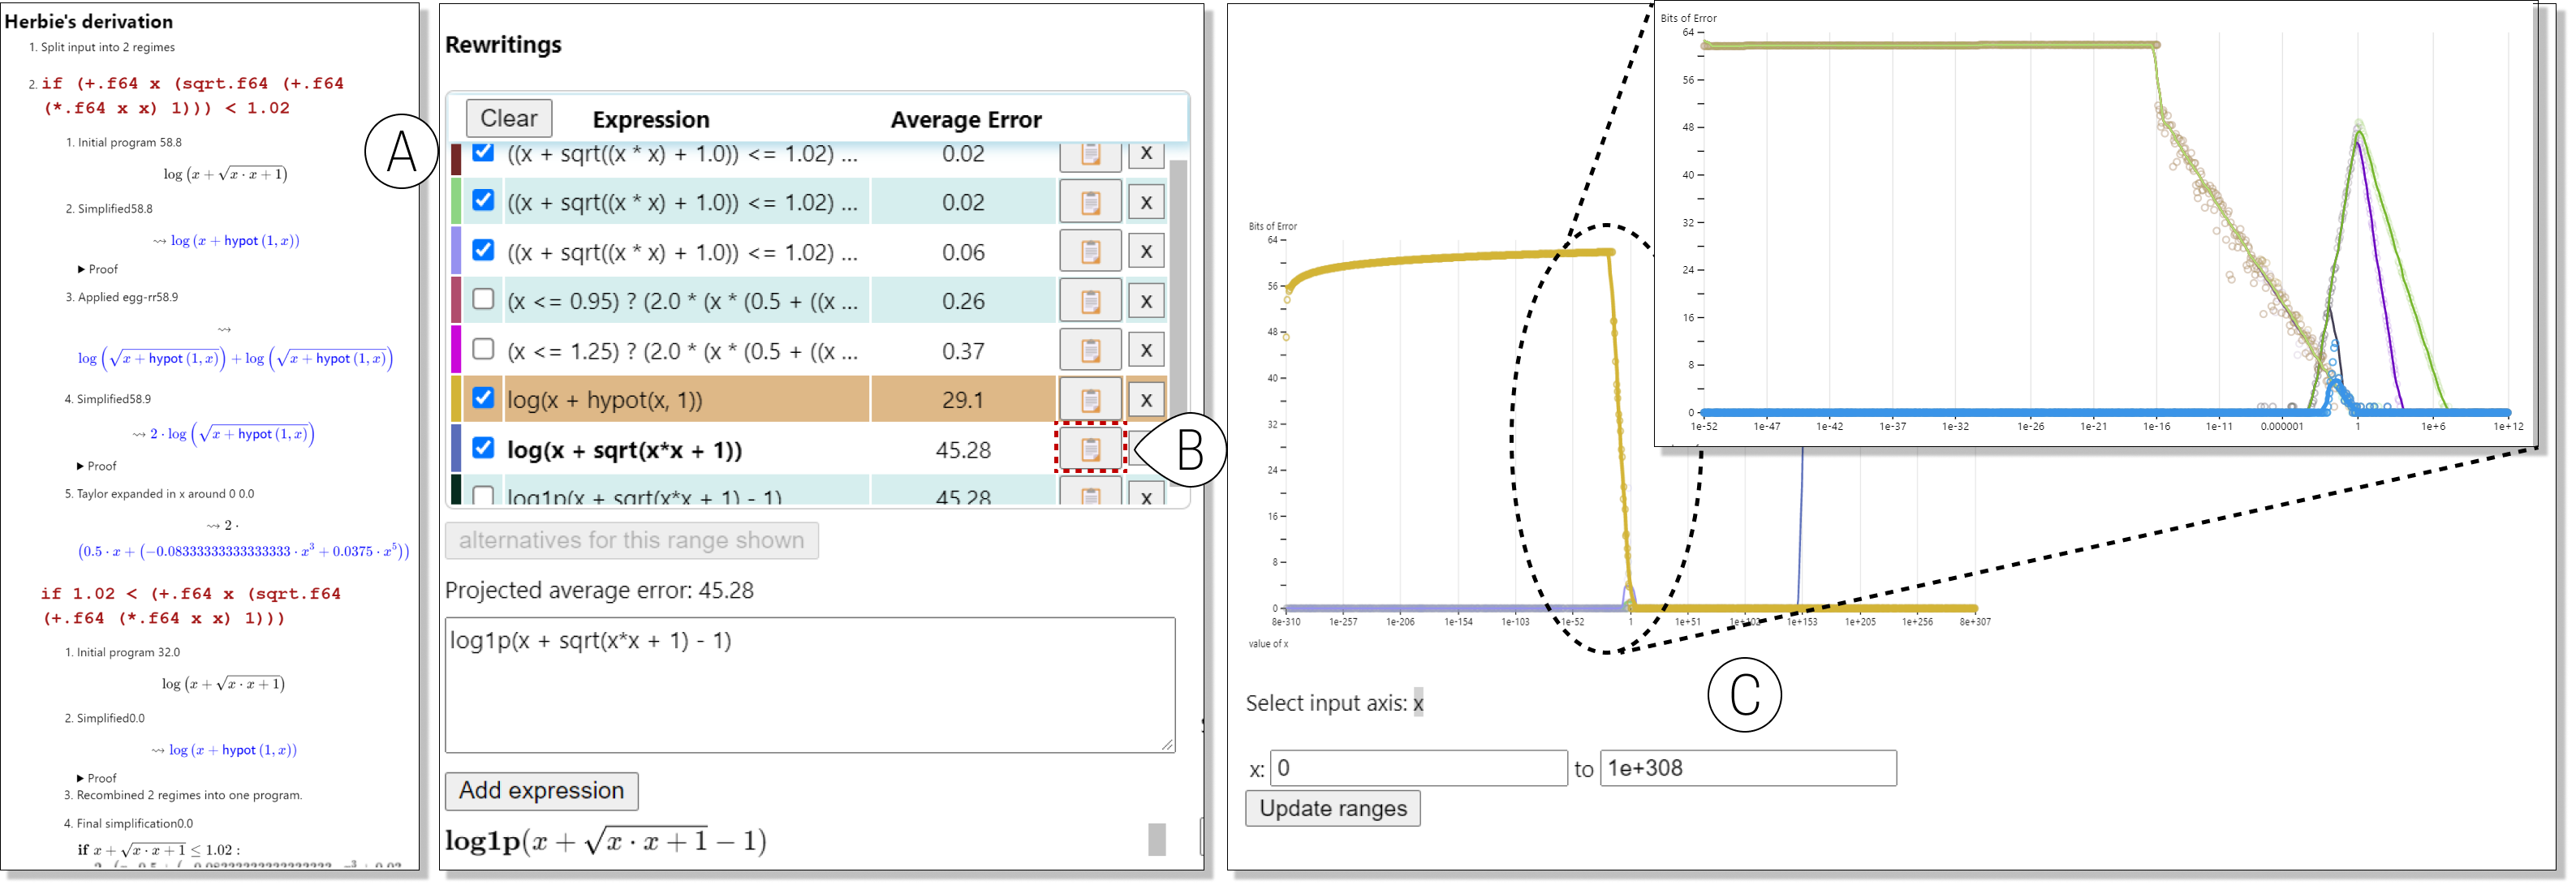
\includegraphics[width=\linewidth]{figures/tuning.png}
  \caption{Tuning. 
  The user can use derivations (A) to help them understand Herbie-generated rewritings.
  Each expression can be copied using the copy button (B) for easy editing of
    existing rewritings.
  The user can use the input range editor (C) to ``zoom in'' on critical ranges---%
    i.e., resample and reanalyze all expressions on a new range. 
    Above, the user has tried rounding some of an expression's constants 
    after zooming.
  }
  \label{fig:tuning}
\end{figure*}

To fix this new-found problem,
  Alex continues to test new rewritings
  using the expression edit box.
Since, at this point, Alex has already found
  many quite-accurate rewritings,
  they choose to modify an existing rewriting
  using the copy-to-clipboard button (\Cref{fig:tuning}B).
This allows Alex to easily make small adjustments,
  such as raising or lowering the threshold 
  by rewriting the branch condition,
  and see how that affects the inputs they have focused on.
Alex may not always tune expressions for accuracy;
  they might instead simplify rewritings to make them run faster,
  or make modifications to improve readability and maintainability.
In those cases, the error graph allows Alex to validate
  that error has not increased unacceptably.
Finally, Alex has tuned the expression to their liking,
  so they use the copy-to-clipboard button
  to copy the final expression %into their IDE
  and insert it into their program.

Reviewing these steps,
  Alex
  used a three-step floating-point error improvement workflow:
  diagnosing the sources of floating-point error;
  generating candidate solutions to these source of error;
  and then tuning and validating the resulting solution
  until it met their accuracy, performance, and maintainability goals.
The entire process was orchestrated
  through Odyssey's table of rewritings and error plot,
  which track the various rewritings Alex already considered
  and allow Alex to easily compare rewritings over the input range.
Odyssey additionally provided convenient ways
  to leverage the automated error-improvement tool Herbie,
  including invoking Herbie, visualizing internal heuristics,
  and presenting derivations.
Combined, these features allow Alex
  to focus on higher-level concerns such as accuracy-improving rewrites
  and acceptable trade-offs between their goals.
